\chapter{Einleitung}
\label{cha:Einleitung}
In dieser Seminararbeit wird das Thema Lerntheorien mit speziellem Bezug auf die Theorien Kognitivismus, Konnektivismus und Konstruktivismus behandelt. Diese Arbeit entstand im Zeitraum November 2015 bis Januar 2016 im Zuge des Integrationsseminar zu ausgewählten Themen der Wirtschaftsinformatik im fünften Semester. In dieser Einleitung soll zu Beginn auf das Lernen im Allgemeinen eingegangen werden.

\section{Lerntheorie}
\label{sec:Lerntheorie}
Lerntheorien befassen sich mit den in Theorien oder gar Gesetzmäßigkeiten gegossenen Ergebnissen aus Experimenten zur Erforschung von Lernen und Gedächtnis. Lernen wird von Irle als der Prozess des Informationserwerbs bezeichnet und wird von ihr abgegrenzt gegen das Gedächtnis. Dieses stehe für die Speicherung und Reproduzierung des Erlernten. \cite[]{Irle.1986}

Lerntheorien beschäftigen sich also damit, wie ein Mensch lernt. \cite{Reinmann.2013} Es existieren einige Lerntheorien, aber es gibt zur Zeit in der Wissenschaft keine etablierte Ansicht über das Zusammenspiel dieser, da sie oft als konkurrierend angesehen werden. \cite[S. 172 - 173]{Weinert.1996} Dieses konkurrierende System an Lerntheorien löst sich aber perspektivisch auf \cite{WittKerres.2002} und man geht dazu über Lerntheorien zweckbezogen gegeneinander aufzuwiegen. \cite{Reinmann.2013}

\section{Modelle didaktischer Aufbereitung}
\label{sec:Lernmodelle}
Bevor der Lernende Wissen aufnehmen kann, muss dieses allerdings erst aufbereitet werden und so 'zu ihm hingebracht' werden. Dies findet über Lehrmedien statt. Über die Art und Weise, welche Funktion diese Lehrmedien genau haben sollen, gibt es unterschiedliche Auffassungen.

\subsection{Kopiermodell}
\label{sub:Kopiermodell}
Gemäß dem Kopiermodell (siehe Graphik \ref{fig:Kerres2001_Kopiermodell})wird das zu erlernende "Wissen von Sachexpert/innen auf ein Medium übertragen werden und von da aus dem Lernenden präsentiert" \cite[S. 146]{Kerres.2001}. Dies führt zu der Annahme, dass das Medium und nicht der Lehrende präsentiert. Außerdem impliziert es die Gleichheit von Lehr- und Wissensinhalten.

Der Name Kopiermodell rührt daher, dass nach diesem didaktischen Modell Lernen nur das Kopieren von Wissen in das Gedächtnis darstellt und eine derartige 1:1 Kopie möglich und sinnvoll ist. \cite[S. 145 - 146]{Kerres.2001}

\begin{figure}[h]
	\centering
	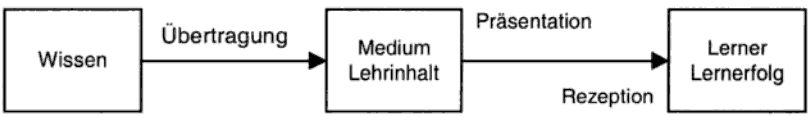
\includegraphics[width=0.6\textwidth]{Abbildungen/Kerres2001_Kopiermodell.PNG}
	\caption{Medien als Übermittler von Lehrinhalten. \cite[S. 146]{Kerres.2001}}
	\label{fig:Kerres2001_Kopiermodell}
\end{figure}

\subsection{Lernen durch Anregung}
\label{sub:LernenDurchAnregung}
Das Kopiermodell gilt aufgrund neuer Erkenntnisse über die menschliche Art zu Lernen und Informationen aufzunehmen als veraltet.
In dem nun beschriebenen alternativen Modell sollen die Lernmedien vielmehr das aktive Lernen anregen, als nur die Lerninhalte wiedergeben. 
Dazu soll das zu vermittelnde Wissen eben in diese anregende Form transformiert werden. (siehe Graphik \ref{fig:Kerres2001_LernenDurchAnregung}) Diese Form soll neben der einfachen Aufnahme des Wissens auch zur Interaktion mit Mitlernenden und zur eigenen Aktion aufrufen. Beides soll die Intensität der Auseinandersetzung mit dem Lernstoff erhöhen. \cite[S. 147 - 148]{Kerres.2001}
\begin{figure}[h]
	\centering
	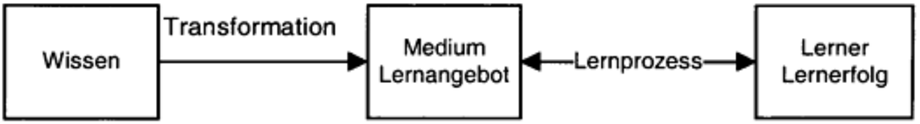
\includegraphics[width=0.6\textwidth]{Abbildungen/Kerres2001_LernenDurchAnregung.PNG}
	\caption{Medien als Angebot zur Anregung von Lernprozessen . \cite[S. 147]{Kerres.2001}}
	\label{fig:Kerres2001_LernenDurchAnregung}
\end{figure}